% Created 2016-08-10 Wed 13:49
\documentclass[11pt]{article}
\usepackage[utf8]{inputenc}
\usepackage[T1]{fontenc}
\usepackage{fixltx2e}
\usepackage{graphicx}
\usepackage{grffile}
\usepackage{longtable}
\usepackage{wrapfig}
\usepackage{rotating}
\usepackage[normalem]{ulem}
\usepackage{amsmath}
\usepackage{textcomp}
\usepackage{amssymb}
\usepackage{capt-of}
\usepackage{hyperref}
\author{erik}
\date{\today}
\title{Clojure Under the Hood}
\hypersetup{
 pdfauthor={erik},
 pdftitle={Clojure Under the Hood},
 pdfkeywords={},
 pdfsubject={},
 pdfcreator={Emacs 24.5.1 (Org mode 8.3.5)}, 
 pdflang={English}}
\begin{document}

\maketitle
\tableofcontents

\textbf{Clojure Under the Hood}

\begin{itemize}
\item or -
\end{itemize}

\textbf{Everything You Wanted to Know about Clojure*}










( * But Were Afraid to Ask)

\section{Our team had some gaps in our understanding of how Clojure works}
\label{sec:orgheadline1}

This talk intends to cast light on those gaps, in the context of a high-level overview,
which will hopefully serve as a practical reference in addressing under-the-hood
problems in the future.

Clojure development has a lot of ingredients for new developers to digest:
\begin{itemize}
\item the Clojure language
\item Leiningen/Maven
\item Java/JVM
\item Lisp syntax
\item Functional Programming
\item Emacs/other
\end{itemize}

So it's not surprising that it's hard to be clear about where one thing ends and
another begins.

This will avoid discussing leiningen and maven,
to focus on Clojure itself, JVM, and Clojure applications.
It \emph{does} assume some basic working knowledge of Clojure.

I am not an expert, so please correct if you hear something wrong or misleading.

\section{This topic has been sooo covered by others}
\label{sec:orgheadline2}

Here are just some of the many good resources for these topics:

\begin{itemize}
\item Clojure.org
\item Clojure Programming (Chas Emerick)
(much of this content is from his book, highly recommended!)
\item Rich Hickey's "Clojure for Java Programmers Pt 1"
\item Decompiling Clojure (Guillermo Winkler)
Nice explanation of 3 entry points to compiler: compile, load \& eval
\item Life of a Clojure Expression (John Hume)
\item How Clojure Babies Are Made (Daniel Higgenbotham)
\end{itemize}

\section{Some questions that this will try to make easier to answer}
\label{sec:orgheadline3}

\begin{itemize}
\item How do you install Clojure?

\item How is it that Clojure is just another .jar file?
(that Clojure is packaged as one of many dependencies within a delivered appication?)

\item How can Clojure exhibit "interpreted"-like language behavior?
For example, lein uberjar, then change .clj files inside, rerun
and program's runtime behavior has changed.

\item Macros: "built-in" vs. user-defined: how can they have the same status?
\end{itemize}

\section{Clojure and Clojure, what is Clojure?}
\label{sec:orgheadline6}

\subsection{Clojure is written in Java and in the Clojure language itself}
\label{sec:orgheadline4}

Which parts are Java?
\begin{itemize}
\item \textbf{Data structures} (symbol, keyword, vector, etc.)
\item \textbf{Special operators} (def, fn, var, do, let, etc.)
\item \textbf{Bytecode compiler} ASM
\end{itemize}

(The data structures and special operators are in clojure/src/jvm/clojure/lang,
and the bytecode compiler is in clojure/src/jvm/clojure/ASM)

The rest is written in Clojure (clojure/src/clj/clojure), that is,
written using functions and macros that are composed of
those data structures and special operators.

Wait! A bytecode compiler? Yes, Clojure itself includes a bytecode compiler,
so Clojure can load and evaluate Clojure expressions at runtime.

\subsection{Clojure is a jar}
\label{sec:orgheadline5}

Clojure can be downloaded as a jar: clojure-1.9.0-alpha10.jar.
It has .clj \& .class files.

The .clj files have already been compiled to .class files,
so Clojure itself doesn't need to go through compilation.

\section{Clojure at Runtime}
\label{sec:orgheadline10}

\subsection{Java basics}
\label{sec:orgheadline7}

Run a simple java application
(packaged as a jar file, which is mostly bytecode .class files):

\texttt{java -jar HelloWorld.jar}

(executes HelloWorld application contained in jar file)

\subsection{Launch a Clojure REPL}
\label{sec:orgheadline8}

\texttt{java -cp clojure.jar clojure.main}

-cp: add this jar to classpath

(What is a classpath? The search path that the JVM will use when looking
for user-defined classes  and resources. It can include both directories
and .zip archives, including .jar files.)

clojure.main: the entrypoint for Clojure

\subsection{Run a file full of Clojure code as a script}
\label{sec:orgheadline9}

\texttt{java -cp clojure.jar clojure.main /path/to/myscript.clj}

\section{Clojure Compilation Model (a Clojure file)}
\label{sec:orgheadline11}
\hspace*{-4cm}
	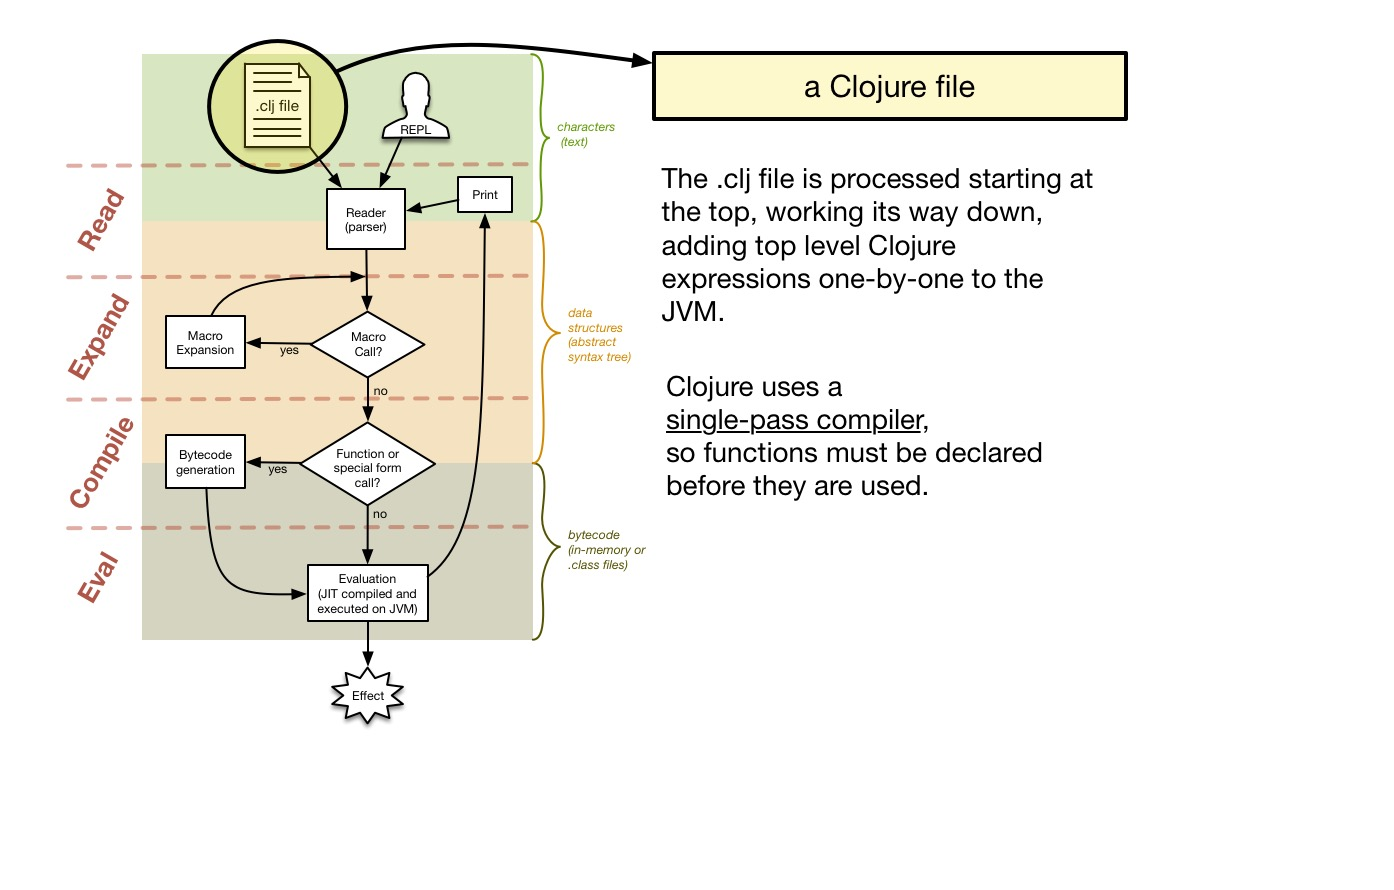
\includegraphics[width=1.9\linewidth]{IMG_0109.JPG}

\section{Clojure Compilation Model (Reader)}
\label{sec:orgheadline12}
\hspace*{-4cm}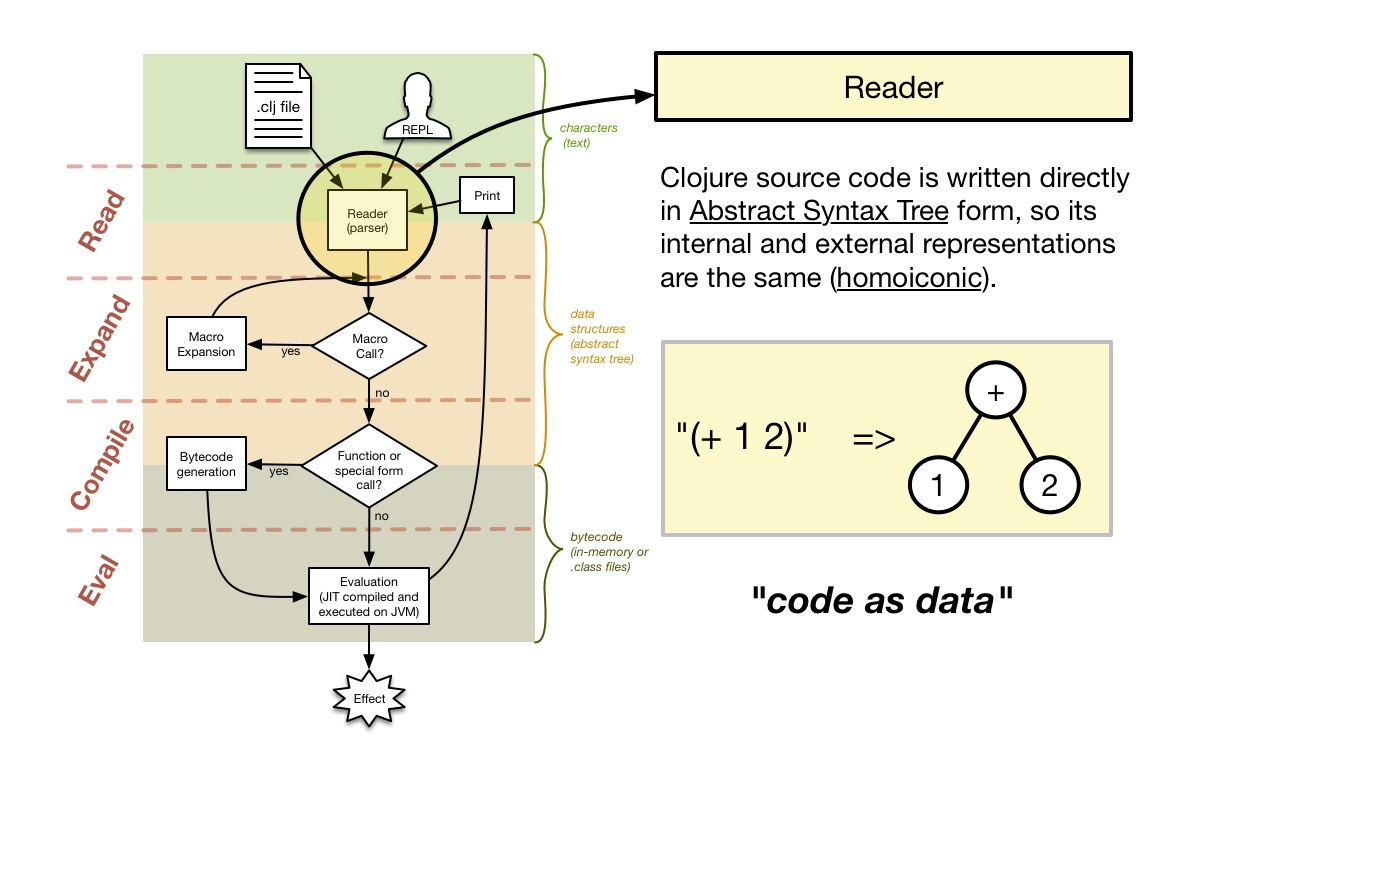
\includegraphics[width=1.9\linewidth]{IMG_0110.JPG}

\section{Clojure Compilation Model (Macro Expansion)}
\label{sec:orgheadline13}
\hspace*{-4cm}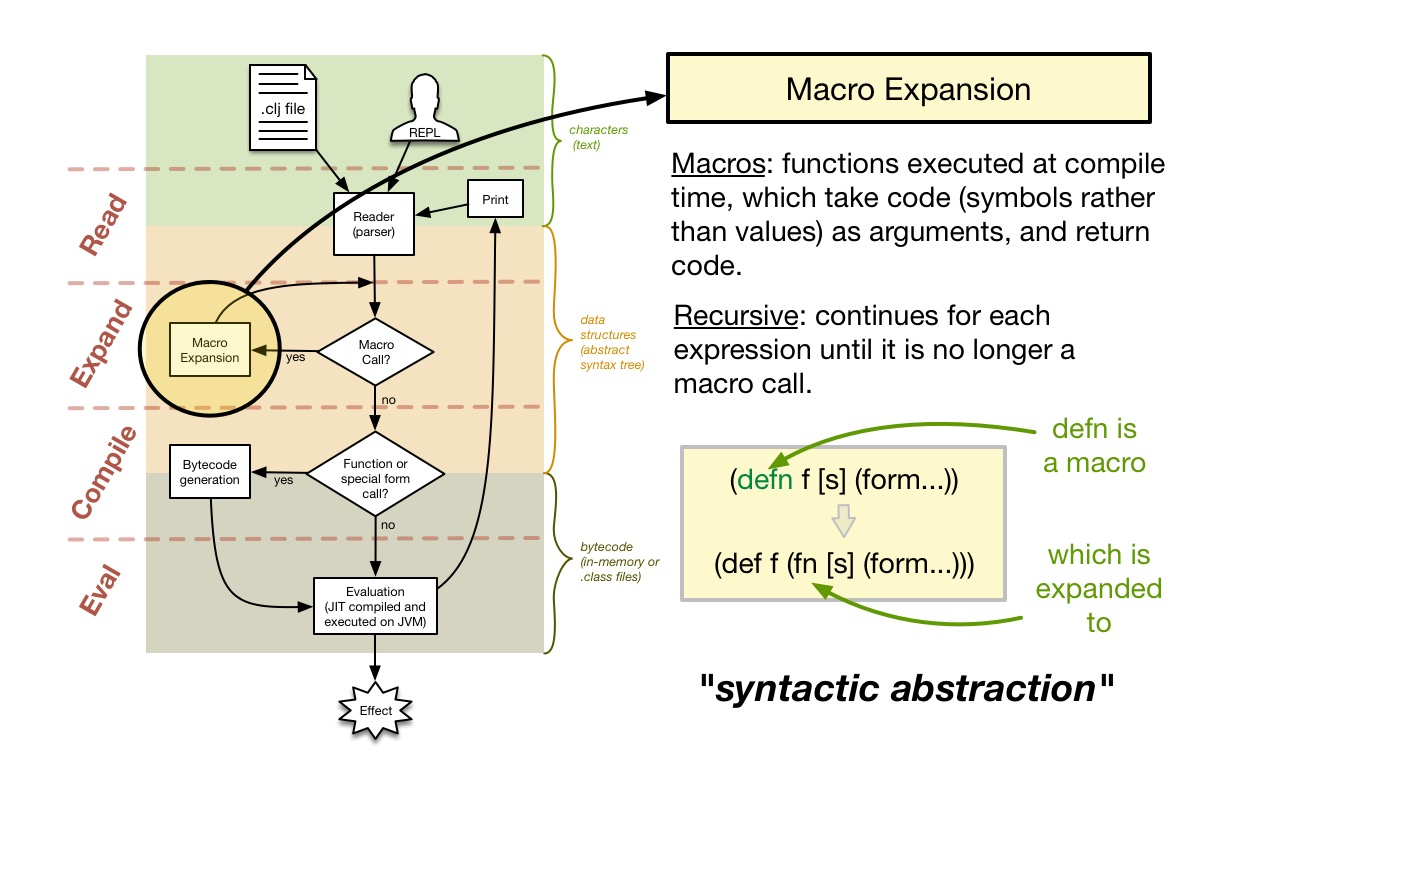
\includegraphics[width=1.9\linewidth]{IMG_0111.JPG}

\section{Clojure Compilation Model (Bytecode Generation)}
\label{sec:orgheadline14}
\hspace*{-4cm}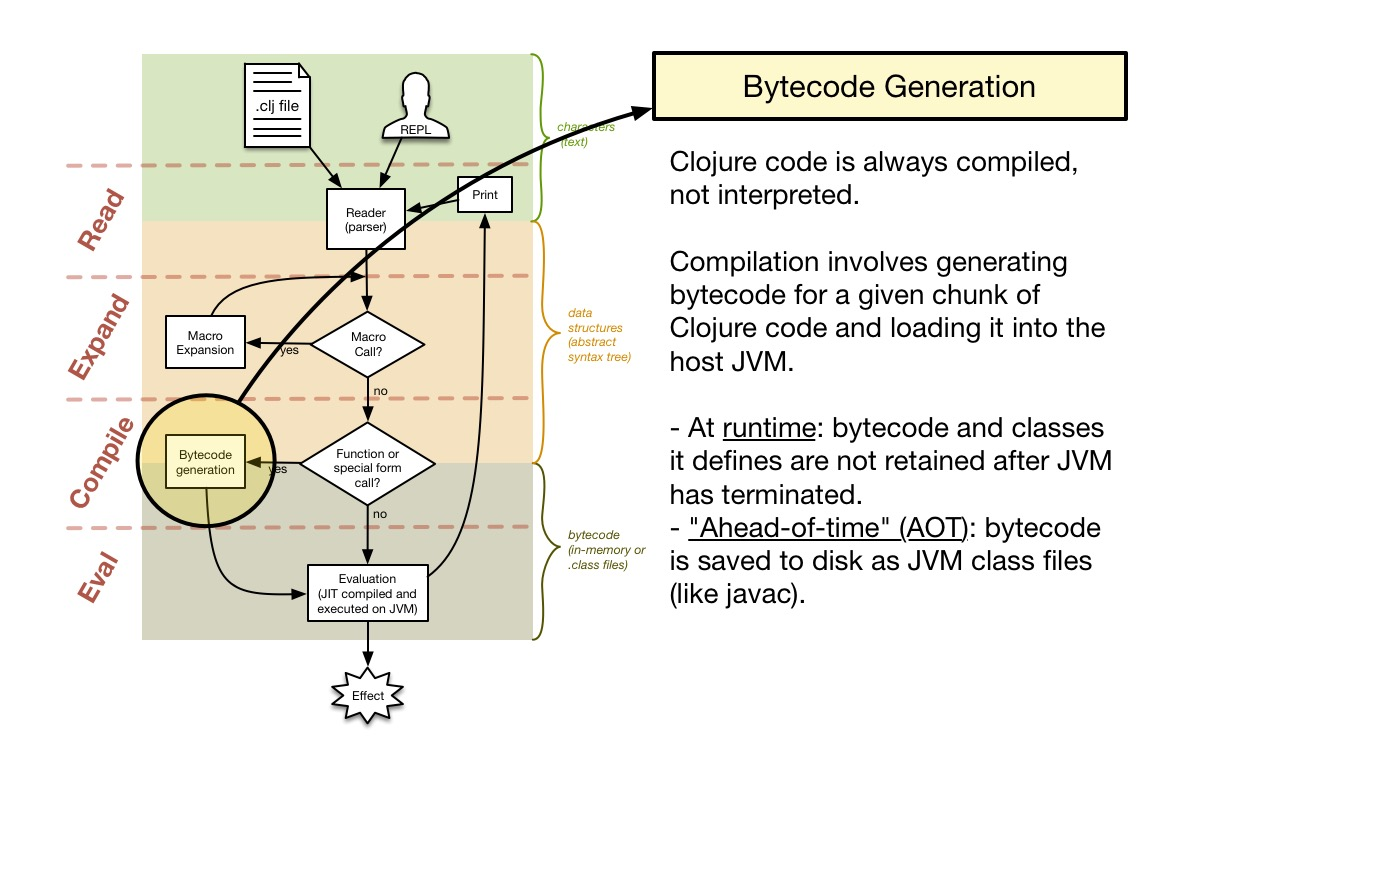
\includegraphics[width=1.9\linewidth]{IMG_0112.JPG}

\section{Clojure Compilation Model (Evaluation)}
\label{sec:orgheadline15}
\hspace*{-4cm}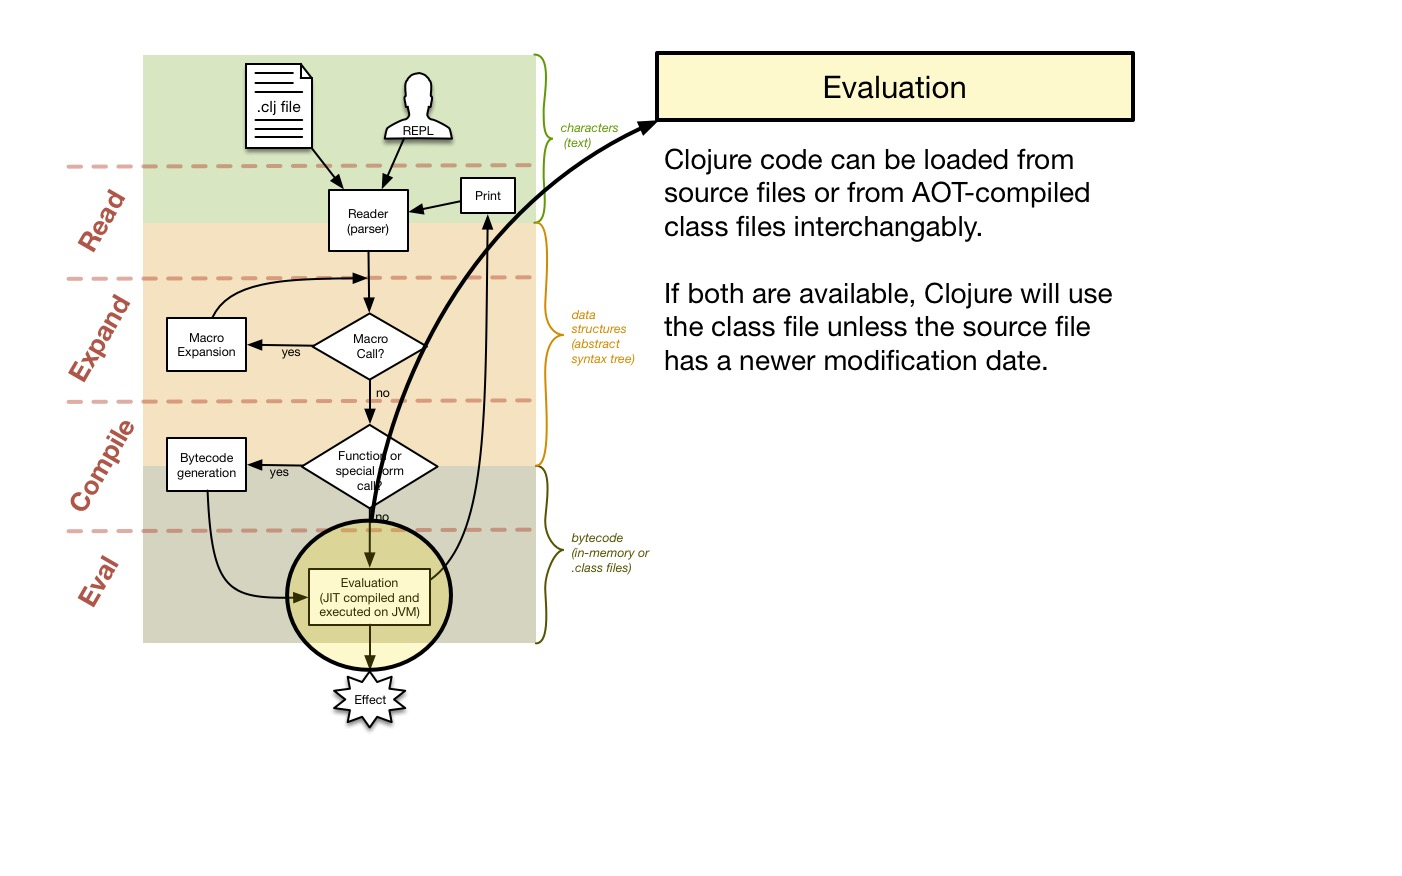
\includegraphics[width=1.9\linewidth]{IMG_0113.JPG}
\end{document}
